%\section{Design}
%\label{chap:design}
%Upon completion of the literature research, a comprehensive understanding of the required components and their functionalities was gained. Utilizing a top-down approach, the design of the \ac{ASIC} commenced, wherein the different functionalities were divided into distinct blocks, as depicted in \autoref{fig:overview}. Initially, these blocks were implemented at a high abstraction level, and subsequently, in greater detail at the semiconductor level. This chapter provides an overview and description of each individual block, shedding light on their specific roles and characteristics.
%%After the literature research was completed it was mostly known which components are needed and how they work. Due to that the design of the \ac{ASIC} was started in a top down approach which means the different functionalities were divided into different blocks as one can see in \autoref{fig:overview}. The blocks itself were firstly implemented in a high abstraction design and afterwards in more detail on semiconductor level. An overview and description of the different blocks can therefore be found in this chapter.
%\begin{figure}[ht]
%	\centering
%	\includegraphics[width = \linewidth]{images/Overview2.drawio.pdf}
%	\caption{Our implementation of cascaded Buck Boost converter with active switches instead of diodes}
%	\label{fig:overview}
%\end{figure}
%
%\subsection{Input}
%The input block includes a POR circuit which makes sure that the circuit turns only on when the input voltage reaches a certain level, a Current reference which provides a input voltage and more or less temperature independent current source, a Band Gap reference which provides a input voltage and temperature independent voltage reference, a oscillator which provides a clock for the FSM.
%\subsubsection{Current source}
%Having a power supply (input voltage) independent current source is one of the key functionality for this project. Due to the fact that current sources are needed for multiple amplifier circuits which are included in function blocks such as the bandgap reference. \newline
%Since this problem was solved already multiple times before it was decided to go with a pre-existing solution/schematic. Lars Kamm therefore provided us with such a circuit, which was afterwards slightly adapted and will be discussed in this section. 
%%\paragraph{Bootstrap definition} 
%%According to \cite{Oxford_dict:bootstrap} bootstrap means: 'To make use of existing resources or capabilities to raise (oneself) to a new situation or state; to modify or improve by making use of what is already present. More recently, as transferred use of sense'\newline
%%For the bootstrap current source this means one creates a current source that is independent of the supply voltage, therefore it's name 'Bootstrap current source'. Note that the term 'Bootstrapping' is used for many completely different circuits as it can be seen in \cite{analog_design_essentials} (p.110).
%\paragraph{Circuit}
%At first glance comprehending a circuit like the one depicted in \autoref{fig:bootstrap4} may present some difficulties. Therefore, the following section provides a step-by-step description of the circuit.
%
%The concept behind the current reference circuit is to leverage the threshold voltage ($V_T$) of the MOSFET, as this parameter remains unaffected by the supply voltage, as indicated in \autoref{eq:mosfet_vt}. To fully comprehend the circuit in \autoref{fig:bootstrap4}, it is essential to grasp basic circuits such as the one shown in \autoref{fig:bootstrap1}. In this particular circuit, the voltage at the gate of $M_0$ is zero, resulting in the absence of a voltage $V_T$ anywhere. In order to establish the desired voltage $V_T$ across the transistor, a certain current $i_D$ must flow. Achieving this can be accomplished by introducing a current mirror into the circuit.
%\begin{figure}[ht]
%	\centering
%	\resizebox{0.3\textwidth}{!}{\subimport{./images/}{bootstrap1.tex}}
%	\caption{Current reference intro}
%	\label{fig:bootstrap1}
%\end{figure}
%When doing that one ends up with \autoref{fig:bootstrap2}. In \autoref{fig:bootstrap2} one has on the gate of $M_0$ the voltage $\Delta V_{GS}+V_T$ whereby $\Delta V_{GS}=V_{GS}-V_T$. When one now increases the ratio of $\frac{W}{L}$   $\Delta V_{GS}$ decreases as one can see from \autoref{eq:mos_ID}, which says: $\Delta V_{GS}=\sqrt{\frac{I_0}{\frac{\mu \cdot C_{ox}}{2} \frac{W}{L}}}$. Therefore when the ratio $\frac{W}{L}$ goes to infinity one would have a stable current through $R$ and a stable voltage on the gate of $M_0$, when one does not consider that $V_T$ is dependent on the temperature and the process. But the issue with the circuit in \autoref{fig:bootstrap2} is that one has a positive feedback loop, which means when the gate voltage on $M_0$ increases the current on $M_1$ and $M_2$ increases too, which increases the gate voltage of $M_0$ even more ($\Rightarrow$ Circuit is unstable). To prevent that one would need to insert an additional mosfet below $M_2$. But as one can see from this circuit one is still dependent on $V_{GS}$ when the ratio of $\frac{W}{L}$ is not infinity. 
%\begin{figure}[ht]
%	\centering
%	\resizebox{0.3\textwidth}{!}{\subimport{./images/}{bootstrap2.tex}}
%	\caption{Current reference example one }
%	\label{fig:bootstrap2}
%\end{figure}
%Let's therefore see if it gets better when one makes sure that the voltage is the same on the gate and the drain of $M_0$. One achieves this with the circuit in \autoref{fig:bootstrap3}. The gate voltage of $M_0$ is $\Delta V_{GS}+V_T$ and on $M_3$ and $M_4$ $2\cdot\Delta V_{GS}+2 \cdot V_T$. Therefore the voltage over R is $\Delta V_{GS}+V_T$. But when one decreases the ratio of $\frac{W}{L}$ of $M_4$ by a factor of 4 the voltage over R reduces to $V_T$ which means one gets rid of $\Delta V_{GS}$ and should therefore be completely independent of $V_{DD}$ \cite{youtube:bias}.
%\begin{figure}[ht]
%	\centering
%	\resizebox{0.3\textwidth}{!}{\subimport{./images/}{bootstrap3.tex}}
%	\caption{Current reference example two}
%	\label{fig:bootstrap3}
%\end{figure}
%\begin{figure}[ht]
%	\centering
%	\resizebox{0.3\textwidth}{!}{\subimport{./images/}{bootstrap4.tex}}
%	\caption{Current reference}
%	\label{fig:bootstrap4}
%\end{figure}
%When one tries to control the temperature dependency too one could add an additional nmos ($M_5$) above R with a $\frac{W}{L}$ x times larger than the one from $M_0$, as it can be seen in \autoref{fig:bootstrap4}. Since one knows that the voltage and the current on the source of $M_3$ and $M_4$ is the same one can write the following equations:
%$$
%\begin{aligned}
%	I_R=\frac{U_R}{R}\\
%	I_{S_{M_0}}=I_{S_{M_5}}\\
%	\sqrt{\frac{I_{S_{M_0}}}{\frac{\mu \cdot C_{ox}}{2}\frac{W}{L}\textcolor{gray}{\left(1+\lambda V_{DS}\right)}}}+V_T=\sqrt{\frac{I_{S_{M_5}}}{\frac{\mu \cdot C_{ox}}{2}\frac{W}{L}\textcolor{gray}{\left(1+\lambda V_{DS}\right)}\cdot x}}+V_T+U_r
%\end{aligned}
%$$
%The result of this equation is then (when one neglects the trivial solution where $I_{S_{M_0}}=I_{S_{M_5}}=0$ and the channel length modulation):
%$$
%I_{S_{M_0}}=I_{S_{M_5}}=\frac{2 \cdot \left(x\pm2\sqrt{x}+1\right) }{\beta\cdot\frac{W}{L}\cdot R^2 \cdot x} \text{ \textcolor{blue}{ !}}
%$$
%$$
%U_R=\frac{2 \cdot \left(x\pm2\sqrt{x}+1\right) }{\beta\cdot\frac{W}{L}\cdot R \cdot x} \text{ \textcolor{blue}{ !}}
%$$
%\textcolor{blue}{One solution from the equations above is an extraneous solutions.} The solutions that are really correct are: $I_{S_{M_0}}=I_{S_{M_5}}=\frac{2 \cdot \left(x-2\sqrt{x}+1\right) }{\beta\cdot\frac{W}{L}\cdot R^2 \cdot x}$ and $
%U_R=\frac{2 \cdot \left(x-2\sqrt{x}+1\right) }{\beta\cdot\frac{W}{L}\cdot R \cdot x}$.
%As one can see from those equations the current is depending on the factor of x and R one can therefore set it with setting x and R respectively. Furthermore it's worth to mention that R has a positive temperature coefficient and $V_{GS}$ a negative one. Therefore when the temperature increases the resistance $R$ gets higher while $V_{GS}$ gets lower. Due to that one could chose R and x in such a way that the circuit is more or less temperature independent. Due to the fact the amplifiers in the other circuits are also temperature dependent one chooses the ratio in such a way the the amplifiers are in the end not temperature dependent. But since this goes really deep into semiconductor physics no formulas for the temperature dependency of this circuits were derived. Nevertheless the simulation results were verified with the temperature independent equations which have shown that the calculations and simulations are quite similar.
%
%%$$
%%V_{\text {taw }}=\frac{k T}{q}=86.2 \frac{\mu V}{K} T
%%$$
%%One can now simplify the the equations to the following formula:
%%$$
%%\sqrt{\frac{I_{S_{M_0}}}{\frac{\mu \cdot C_{ox}}{2}\frac{W}{L}}}+V_T=\sqrt{\frac{I_{S_{M_0}}}{\frac{\mu \cdot C_{ox}}{2}\frac{W}{L}\cdot x}}+V_T+I_{S_{M_0}} \cdot R
%%$$
%%$$
%%\frac{I_{S_{M_0}}}{\frac{\mu \cdot C_{ox}}{2}\frac{W}{L}}=\frac{I_{S_{M_0}}}{\frac{\mu \cdot C_{ox}}{2}\frac{W}{L}\cdot x}+\sqrt{\frac{I_{S_{M_0}}}{\frac{\mu \cdot C_{ox}}{2}\frac{W}{L}\cdot x}} \cdot (I_{S_{M_0}} \cdot R)+\left(I_{S_{M_0}} \cdot R \right)^2
%%$$
%%
%%$$
%%a=\left(I_{S_{M_0}} \cdot R \right)^2
%%$$
%%
%%$$
%%b=\frac{I_{S_{M_0}} \cdot (1-x)}{\frac{\mu \cdot C_{ox}}{2}\frac{W}{L}}
%%$$
%%
%%$$
%%c=0
%%$$
%%$$
%%x_{1,2}=\frac{-b \pm \sqrt{b^2-4 a c}}{2 a}
%%$$
%%solve(((ur)/(r))=i00 and i00=i05 and √(((i00)/(((beta)/(2))*wl)))+vt=√(((i05)/(((beta)/(2))*wl*x)))+vt+ur,i00,i05,ur)
%When inserting the values of the circuit one gets the following result:
%
%$$
%I_{S_{M_0}}=I_{S_{M_5}}=\frac{2 \cdot \left(16-2\sqrt{16}+1\right) }{\SI[group-digits=true]{103e-6}{\ampere\per\volt\squared} \cdot16\cdot \SI[group-digits=true]{22.5e-3}{\ohm}^2 \cdot 16}=\SI[group-digits=true]{2.697e-6}{\ampere}
%$$
%$$
%U_R=\frac{2 \cdot \left(16-2\sqrt{16}+1\right) }{\SI[group-digits=true]{103e-6}{\ampere\per\volt\squared} \cdot16\cdot \SI[group-digits=true]{22.5e-3}{\ohm} \cdot 16}=\SI[group-digits=true]{168.554}{\milli\volt}
%$$
%with:
%\begin{description}
%	[font=\normalfont,leftmargin=1.9in,style=multiline]
%	\item[$\beta$]
%	$\qty{103}{\micro\ampere\per\volt\squared}$
%	\item[$R$]
%	\qty{22.5}{\kilo\ohm}
%	\item[$\frac{W}{L}$]
%	8
%	\item[$x$]
%	16
%\end{description}
%This similar to the simulation (simulation\footnote{Simulation result can be found in \autoref{fig:bootstrap_mon} in the appendix}: $\SI[group-digits=true]{4.9}{\micro\ampere}$, calculation: $\SI[group-digits=true]{2.7}{\micro\ampere}$).
%
%
%
%\begin{figure}[ht]
%	\centering
%	
%	\resizebox{1\textwidth}{!}{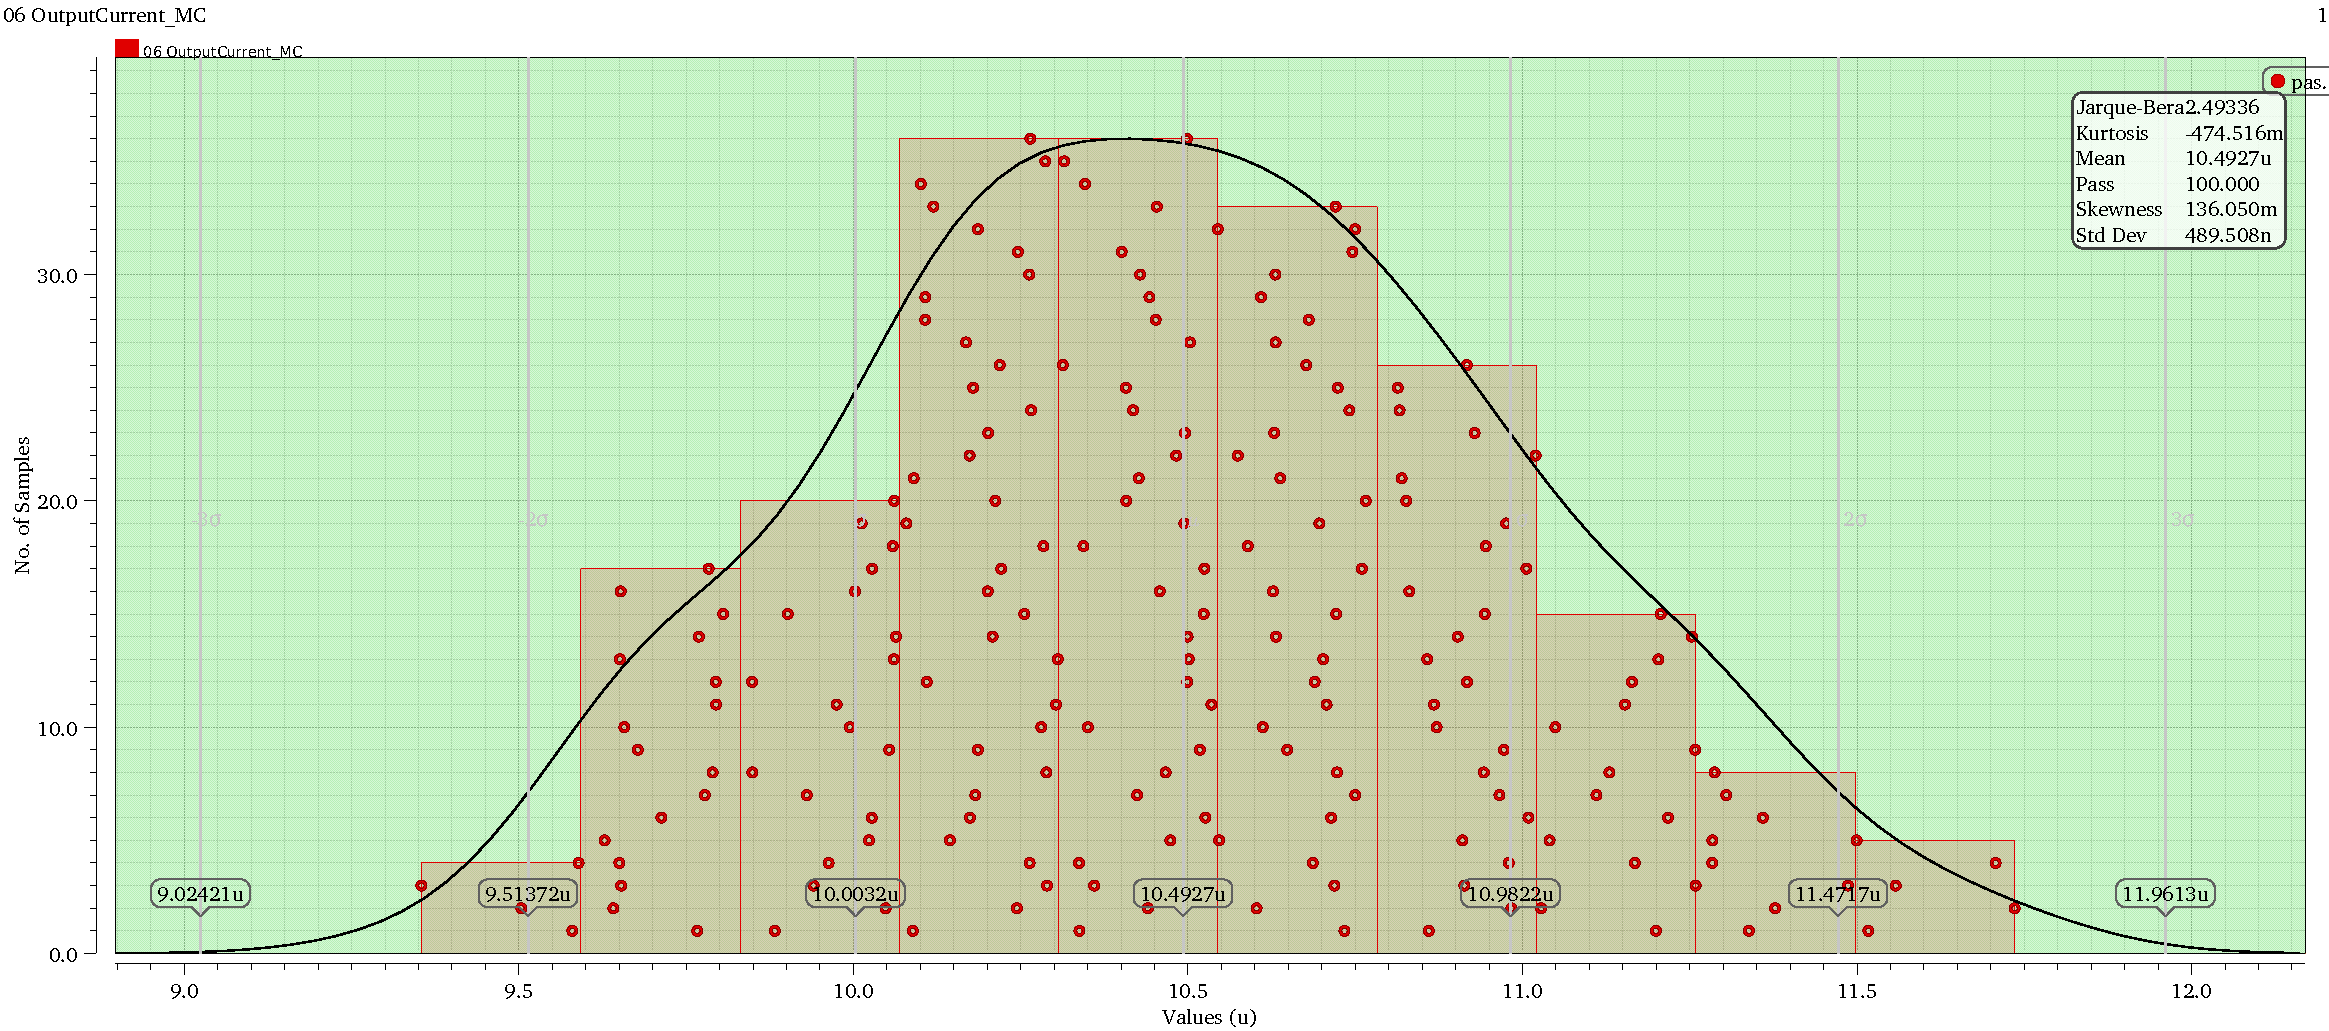
\includegraphics{../ASIC-DESIGN/data/03_Plots/02_Bootstrap/ref_cur_mont.pdf}}
%	\caption{Monte Carlo distribution of Current reference. X-axis shows current through \glqq IPRB0\grqq{} in \autoref{fig:ref_cur_sim_schem} (param.scs=3s, xh035.scs=mcg)}
%	\label{fig:ref_cur_mont}
%\end{figure}
%
%The implemented design on the chip can be seen in \autoref{fig:bootstrap5}. For simplicity one can neglect in a first step M89, M10, M13, M19 and M21. When doing that one sees in \autoref{fig:bootstrap5} the same circuit as in \autoref{fig:bootstrap4} with some additions (M51 and M52 are not needed they were introduced in the layout for a common centroid design). This additions are needed since one has two operating points as one saw before. To be in the right operating point a so called start up circuit is needed which will be explained in more detail. On the left of \autoref{fig:bootstrap5} one finds the enable signal EN and its inverted signal ENN. In turned off state M15 is conducting an therefore M14 discharged, furthermore VB4 is pulled to VDDA which forces the bootsrap to be in state zero (state where no current is flowing). When the circuit is turned on  M8, M9 and M11 are conducting, since their gate voltage is zero which leads to the fact that the node voltage of N2 is pulled to VDDA. Furthermore VB4 is not any more pulled to VDDA. The voltage in N2 causes a current in the Current reference which is mirrored to M5, which charges the capacitor M14 and finally stops N2 to be pulled to VDDA. The Current reference is now in its operating state where current is flowing. This current can then be further mirrored to other components with VB4, VB3, VB2 and VB1.
%\begin{figure}[ht]
%	\centering
%	\includegraphics[width=\textwidth]{../ASIC-DESIGN/data/03_Plots/02_Bootstrap/ref_cur_schem.png}
%	\caption{Current reference Implemented}
%	\label{fig:bootstrap5}
%\end{figure}
%\autoref{fig:ref_cur_sim_schem} shows the testbench used to test the current reference circuit. 
%\begin{figure}[ht]
%	\centering
%	\includegraphics[width=\textwidth]{../ASIC-DESIGN/data/03_Plots/02_Bootstrap/ref_cur_sim_schem.png}
%	\caption{Current reference test bench}
%	\label{fig:ref_cur_sim_schem}
%\end{figure}
%
%
%\autoref{fig:ref_cur_cur} shows the current in dependency of the supply voltage. 
%\begin{figure}[ht]
%	\centering
%	\includegraphics[width=\textwidth]{../ASIC-DESIGN/data/03_Plots/02_Bootstrap/ref_cur_cur.pdf}
%	\caption{Current reference current vs supply voltage}
%	\label{fig:ref_cur_cur}
%\end{figure}
%\autoref{fig:boot_out_res} shows the transresistance of the Input voltage to the output current. It is visible from this plot that the current reference should be operated with a voltage greater than 3.3V to have a input voltage independent current.
%\begin{figure}[ht]
%	\centering
%	\includegraphics[width=\textwidth]{../ASIC-DESIGN/data/03_Plots/02_Bootstrap/ref_cur_tran_res.pdf}
%	\caption{Current reference trans resistance $\frac{\Delta V_{in}}{\Delta I_{out}}$}
%	\label{fig:boot_out_res}
%\end{figure}
%
%\autoref{fig:boot_out_res_2} shows the output resistance of the current reference ($V_4$ in \autoref{fig:ref_cur_sim_schem}) divided by the current that goes into the source of $V_4$ at different voltages. This allows to estimate how many diode voltage one is allowed to use to mirror the reference current. It shows that the voltage of the diode must be at least one 0.8V below the supply voltage.
%\begin{figure}[ht]
%	\centering
%	\includegraphics[width=\textwidth]{../ASIC-DESIGN/data/03_Plots/02_Bootstrap/ref_cur_res.pdf}
%	\caption{Current reference output resistance $\frac{\Delta V_{out}}{\Delta I_{out}}$}
%	\label{fig:boot_out_res_2}
%\end{figure}
%%\begin{figure}[ht]
%%	\centering
%%	\includegraphics[width=\textwidth]{../ASIC-DESIGN/data/03_Plots/02_Bootstrap/09_bootstrap_tb_2.png}
%%	\caption{Current reference test bench two}
%%	\label{fig:bot_tb_schem2}
%%\end{figure}
%
%
%%\begin{figure}[ht]
%%	\centering
%%	\includegraphics[width=\textwidth]{../ASIC-DESIGN/data/03_Plots/02_Bootstrap/06_test_results.png}
%%	\caption{Current reference test}
%%	\label{fig:boot_test}
%%\end{figure}
%The summarized specification of the block can be found in \autoref{tab;bootstrap}.
%\begin{longtable}{|p{3.5cm}|p{3.5cm}|p{3.5cm}|p{3.5cm}|}
%	\hline
%	\rowcolor{lightgray}
%	\textbf{Description} &\textbf{Min}  &\textbf{Max} & \textbf{Unit} \\ \hline
%	
%	Reference current & 8.4 & 13.5 &\qty{}{\micro\ampere} \\ \hline
%	Current consumption & 50 & 81 & \qty{}{\micro\ampere} \\ \hline
%	Min voltage (voltage where the trans resistance ($\frac{\Delta V_{in}}{\Delta I_{out}}$) is higher than \qty{1}{\mega\ohm}) & 3& 3.33 & \qty{}{\volt} \\ \hline
%	\caption{Current reference characteristics} % needs to go inside longtable environment
%	\label{tab:booststrap}
%\end{longtable}
%
%\clearpage
%
%\subsubsection{Bandgap}
%For the \href{https://youtu.be/ncZzxvG4XOM}{Bandgap reference} a given implementation of a 3.3V circuit from X-Fab was taken and adapted for the 5V technology. The final design can be seen in \autoref{fig:bandgap_schem}.
%
%\begin{figure}[ht]
%	\centering
%	\includegraphics[width=\textwidth]{../ASIC-DESIGN/data/03_Plots/03_Bandgap/band_gap_schem.png}
%	\caption{Bandgap schematic}
%	\label{fig:bandgap_schem}
%\end{figure}
%
%For the test the schematic in \autoref{fig:bandgap_tb_schem} was used, where EN is set to 5V and ENN to 0V furthermore VddA was sweept from 0V to 5.5V
%\begin{figure}[ht]
%	\centering
%	\includegraphics[width=\textwidth]{../ASIC-DESIGN/data/03_Plots/03_Bandgap/band_gap__tb_schem.png}
%	\caption{Bandgap testbench}
%	\label{fig:bandgap_tb_schem}
%\end{figure}
%
%\autoref{fig:bandgap_voltage_vs_supplyv} shows that the bandgap voltage is quite stable over the corners, but  slight variations can be seen in \autoref{fig:bandgap_voltage_mc} the montecarlo simulation. Since the output voltage of the DC/DC converter is anyway exactly set by a external resistor only the variance over the temperature and supply voltage plays a major role. Which is very low as can be seen in \autoref{fig:bandgap_voltage_vs_supplyv} and \autoref{fig:bandgap_voltage_vs_temp}.
%\begin{figure}[ht]
%	\centering
%	\includegraphics[width=\textwidth]{../ASIC-DESIGN/data/03_Plots/03_Bandgap/band_volt_volt.pdf}
%	\caption{Bandgap voltage vs supplyvoltage}
%	\label{fig:bandgap_voltage_vs_supplyv}
%\end{figure}
%\begin{figure}[ht]
%	\centering
%	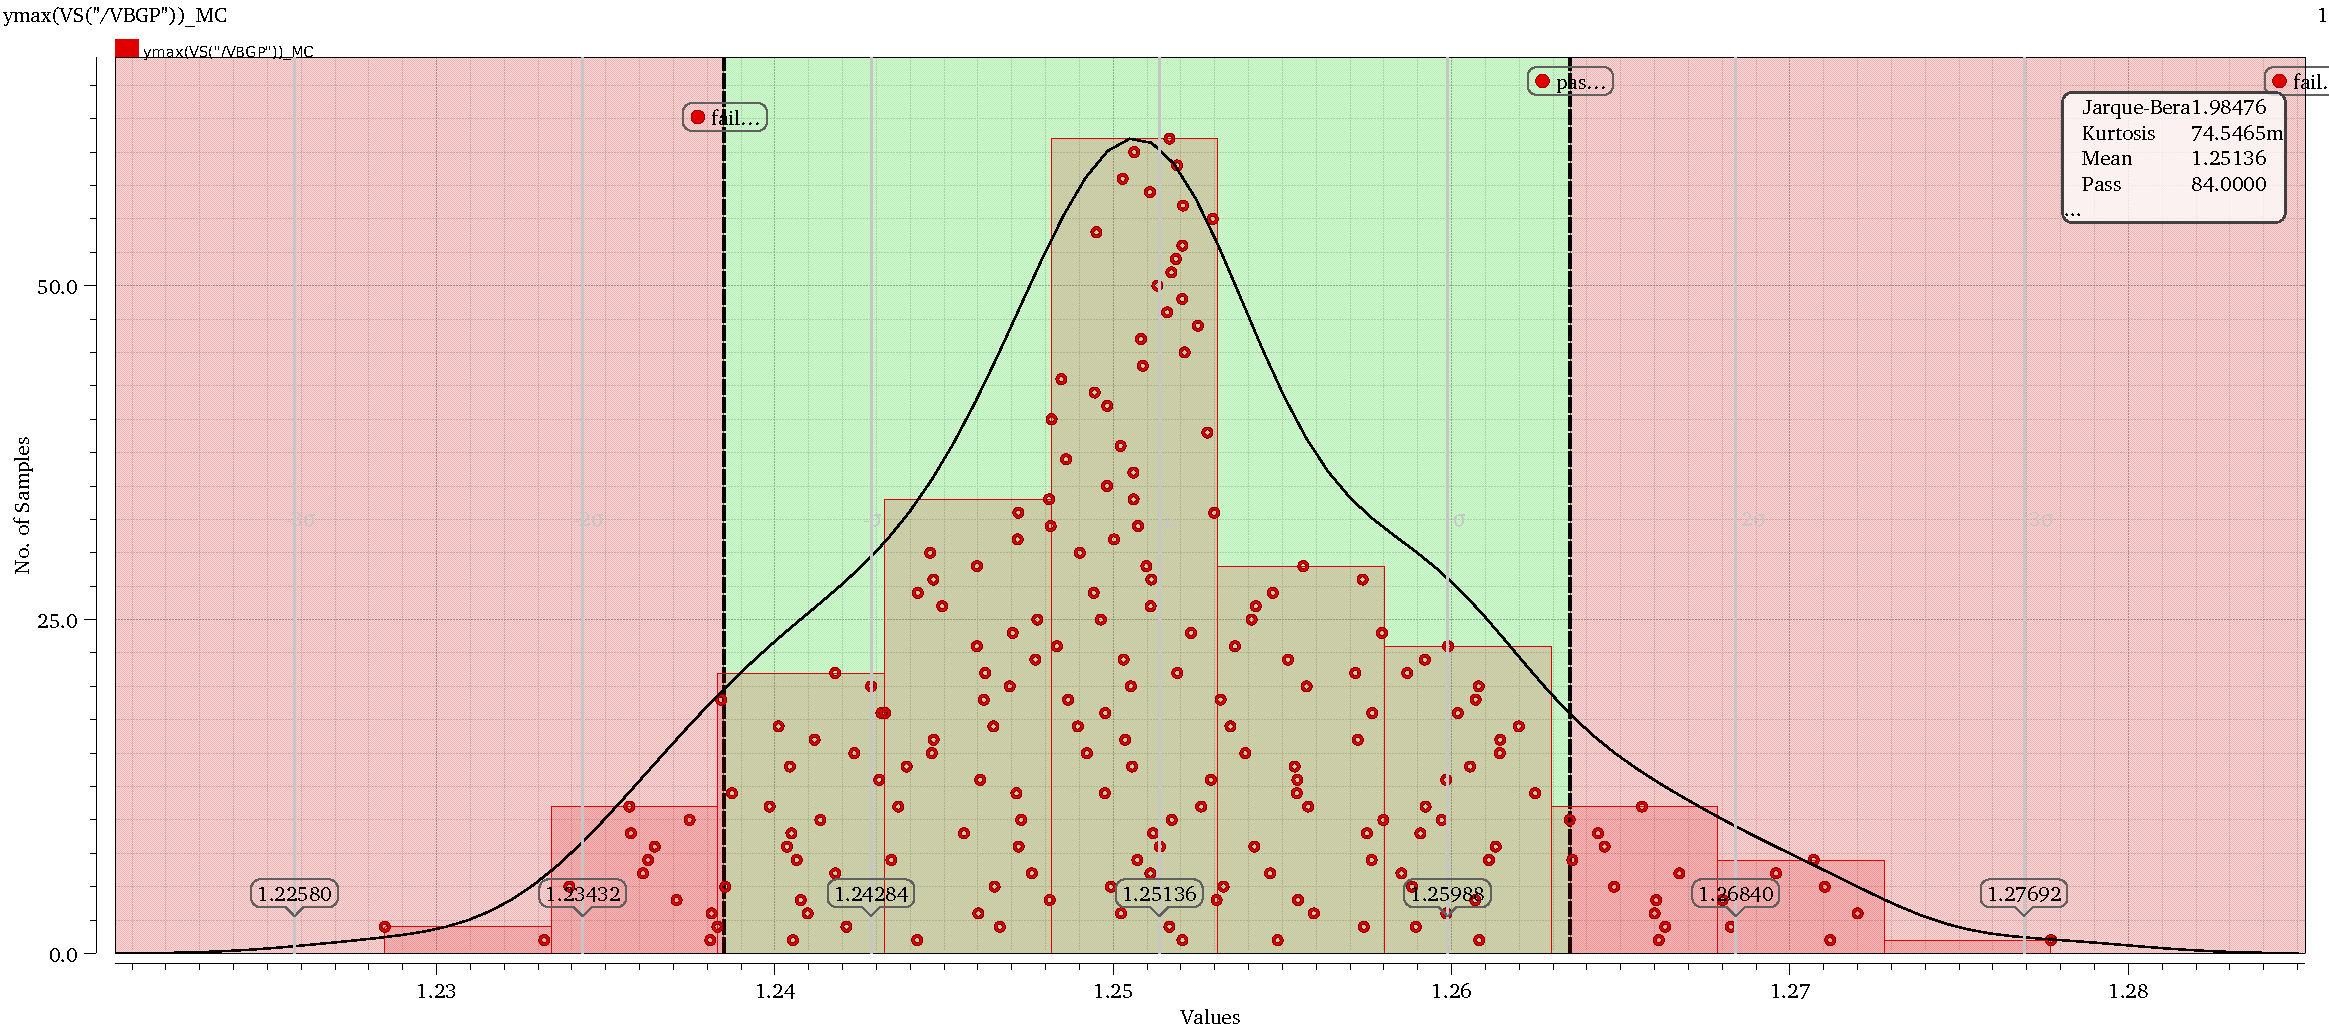
\includegraphics[width=\textwidth]{../ASIC-DESIGN/data/03_Plots/03_Bandgap/band_volt_mc.pdf}
%	\caption{Bandgap voltage Montecarlo simulation (param.scs=3s, xh035.scs=mcg)}
%	\label{fig:bandgap_voltage_mc}
%\end{figure}
%
%\begin{figure}[ht]
%	\centering
%	\includegraphics[width=\textwidth]{../ASIC-DESIGN/data/03_Plots/03_Bandgap/04_Test.png}
%	\caption{Bandgap test output}
%	\label{fig:bandgap_test}
%\end{figure}
%\autoref{fig:bandgap_voltage_vs_temp} shows the dependency of the bandgap voltage vs the temperature.
%\begin{figure}[ht]
%	\centering
%	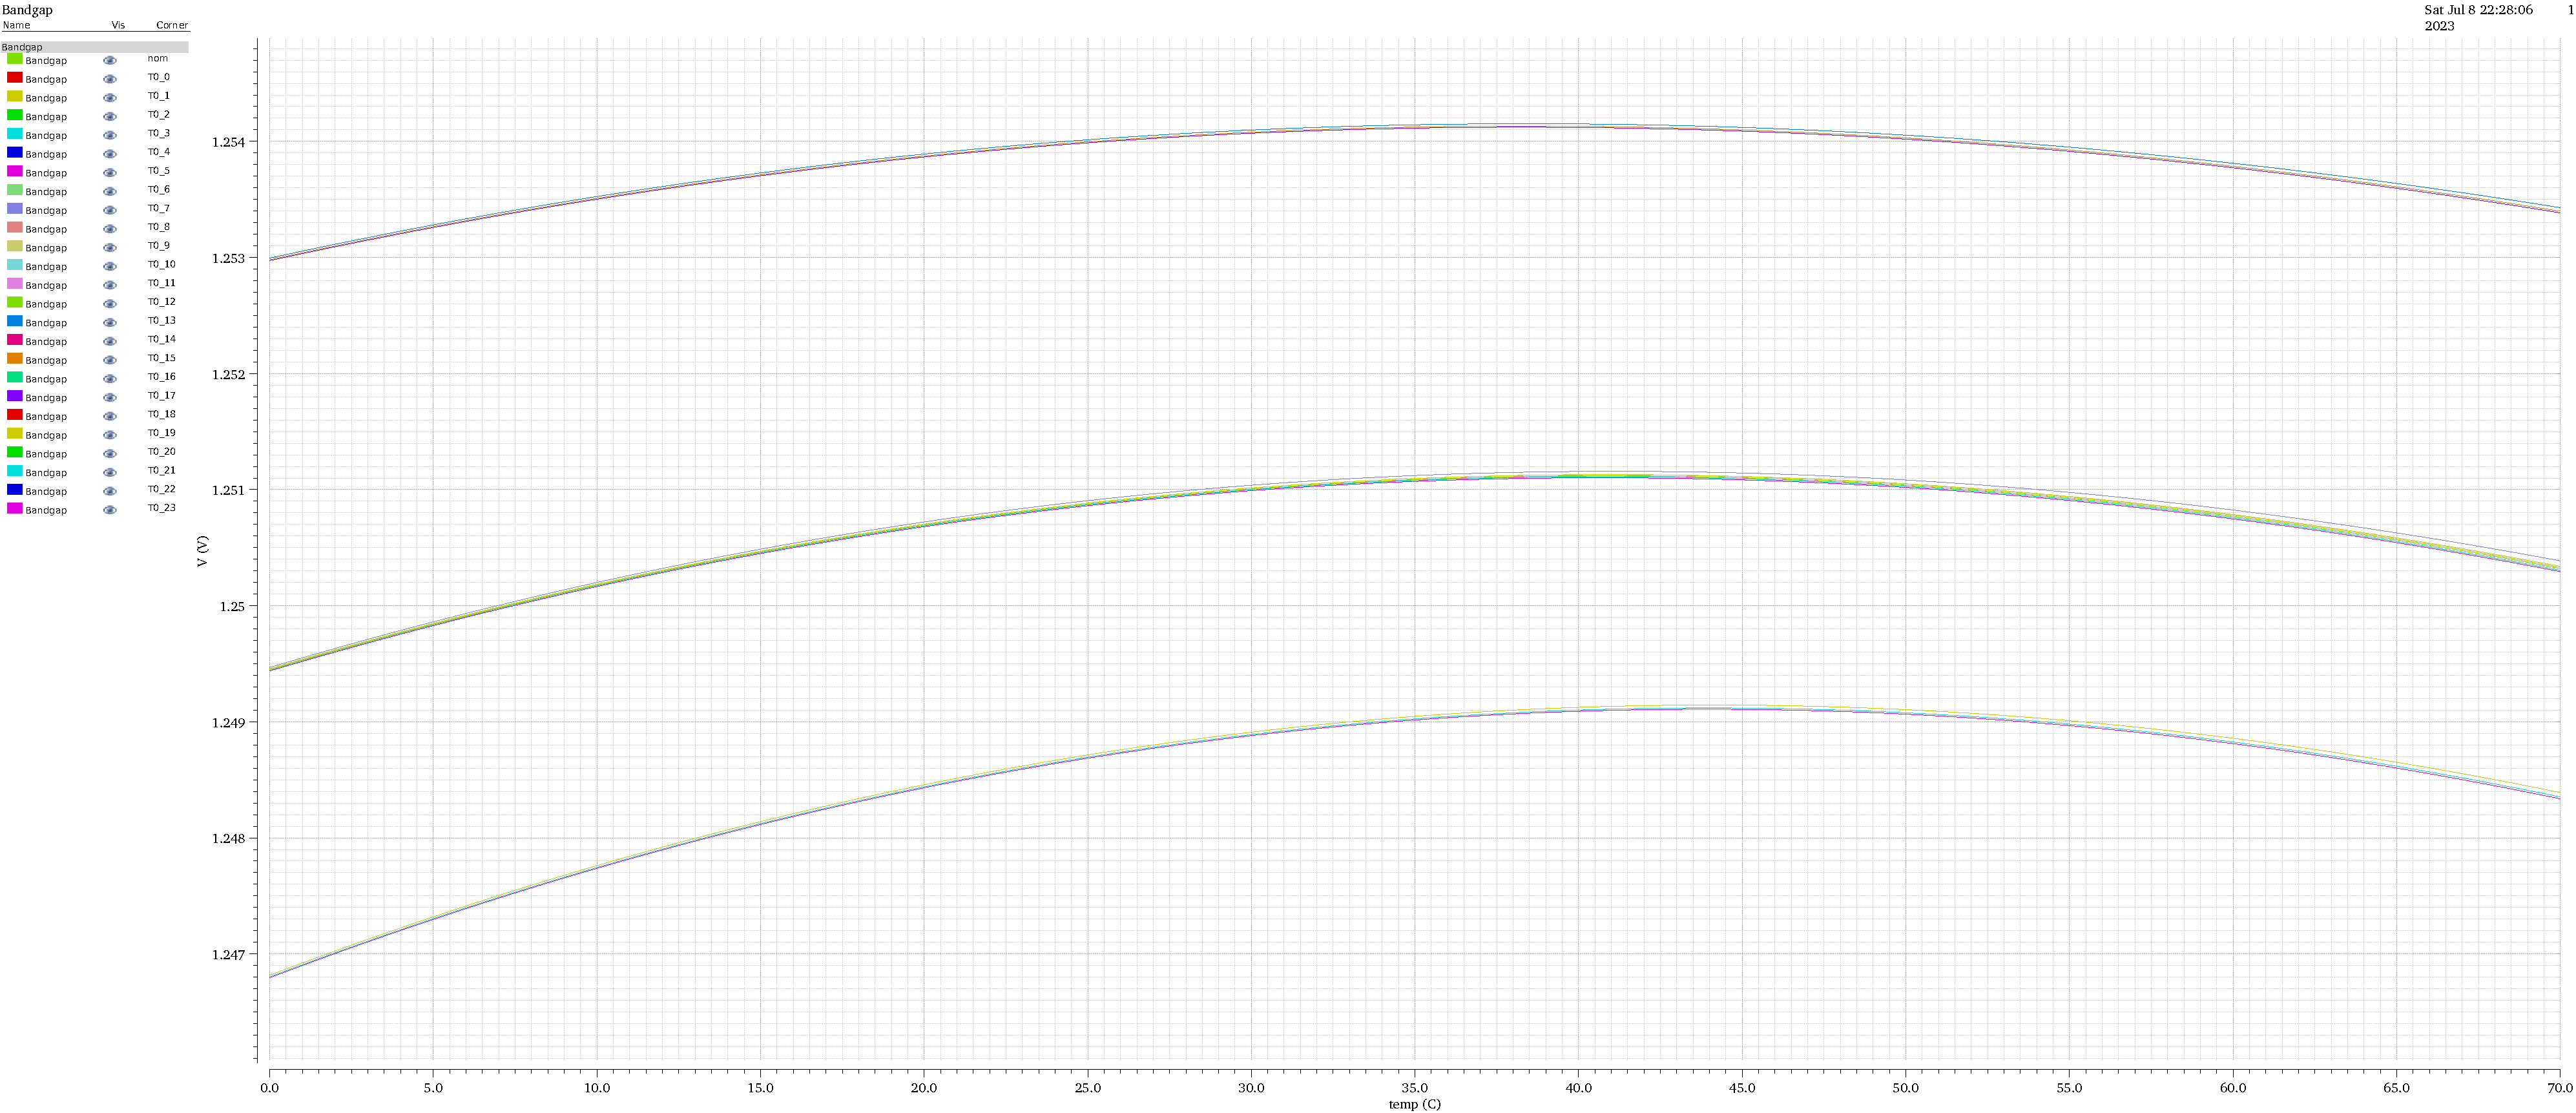
\includegraphics[width=\textwidth]{../ASIC-DESIGN/data/03_Plots/03_Bandgap/band_volt.pdf}
%	\caption{Bandgap voltage vs temperature}
%	\label{fig:bandgap_voltage_vs_temp}
%\end{figure}
%
%\autoref{tab:bandgap} Show the characteristics of the bandgap design used in this project.
%\begin{longtable}{|p{3.5cm}|p{3.5cm}|p{3.5cm}|p{3.5cm}|}
%	\hline
%	\rowcolor{lightgray}
%	\textbf{Description} &\textbf{Min}  &\textbf{Max} & \textbf{Unit} \\ \hline
%	
%	Bandgap voltage & 1.226 & 1.277 &\qty{}{\volt} \\ \hline
%	Current consumption & 16.73 & 23.53 & \qty{}{\micro\ampere} \\ \hline
%	Min voltage & 2.3& 2.9 & \qty{}{\volt} \\ \hline
%	\caption{Bandgap characteristic} % needs to go inside longtable environment
%	\label{tab:bandgap}
%\end{longtable}
%\clearpage
%
%\subsubsection{Oscillator}
%For the digital part of the circuit there is a clock required to process the data received over the SPI. \footnote{It was decided to generate an internal clock although it would have been possible to build a finite state machine which uses the SPI signal only to read and write the registers.} Since the SPI standard does not define a certain clock speed the frequency generated in the \ac{ASIC} plays a minor role. Due to that it was decided to generate the clock with a sawtooth generator (a capacitor gets charged with a certain current and as soon as it reaches a threshold it gets discharged) due to the fact that this approach is very easy to implement and fully compatible with the CMOS process used.
%The design used can be seen in \autoref{fig:osc_schem}.
%\begin{figure}[ht]
%	\centering
%	\includegraphics[width=\textwidth]{../ASIC-DESIGN/data/03_Plots/04_Clock/01_Oscillator_schematic.png}
%	\caption{Oscillator schematic}
%	\label{fig:osc_schem}
%\end{figure}
%As the name tells it delivers a define current to the circuit, which is used to charge the capacitor M7. As soon as the voltage at the drain of M0 reaches a certain threshold the smith trigger triggers and discharges the cap over R0. Due to the fact that the cap gets much faster discharged than charged the signal after the smith trigger is only a short impulse. To get a clock with a duty cycle of about 50\% a d-flipflop was added which changes it's value by every impulse. This reduces the clock frequency by a factor of two but allows to achieve the previously mentioned duty cycle.
%
%The test bench used to validate the design can be seen in \autoref{osc_tb}.
%\begin{figure}[ht]
%	\centering
%	\includegraphics[width=\textwidth]{../ASIC-DESIGN/data/03_Plots/04_Clock/02_Oscillator_tb_schematic.png}
%	\caption{Oscillator test bench schematic}
%	\label{fig:osc_tb}
%\end{figure}
%The EN signal was set to 5V and the ENN to 0V whereas the VddA voltage was swept from 0V to 5V. From \autoref{fig:osc_freq_volt} one sees the circuit works from about 3.2V. 
%\begin{figure}[ht]
%	\centering
%	\includegraphics[width=\textwidth]{../ASIC-DESIGN/data/03_Plots/04_Clock/03_oscillator_frequency_vs_voltage_plot_compressed.pdf}
%	\caption{Oscillator frequency vs voltage}
%	\label{fig:osc_freq_volt}
%\end{figure}
%The exact value can be read from \autoref{fig:osc_test}, which says 3.187V.
%\begin{figure}[ht]
%	\centering
%	\includegraphics[width=\textwidth]{../ASIC-DESIGN/data/03_Plots/04_Clock/04_Test.png}
%	\caption{Oscillator test output}
%	\label{fig:osc_test}
%\end{figure}
%The most important Values can be read from \autoref{tab:osc} and further values can be read from \autoref{fig:osc_test}.
%\begin{longtable}{|p{3.5cm}|p{3.5cm}|p{3.5cm}|p{3.5cm}|}
%	\hline
%	\rowcolor{lightgray}
%	\textbf{Description} &\textbf{Min}  &\textbf{Max} & \textbf{Unit} \\ \hline
%	
%	Frequency & 1.15 & 1.7 &\qty{}{\mega\hertz} \\ \hline
%	Current consumption & 35 & 50 & \qty{}{\micro\ampere} \\ \hline
%	Min voltage & 2& 3.187 & \qty{}{\volt} \\ \hline
%	\caption{Specification} % needs to go inside longtable environment
%	\label{tab:osc}
%\end{longtable}
%
%\clearpage
%\subsubsection{POR}
%For the POR circuit an example was provided by Lars Kamm and afterwards adapted, so that it has the right power on voltage and delay time. The final design can be seen in \autoref{fig:por_schem}.
%
%\begin{figure}[ht]
%	\centering
%	\includegraphics[width=\textwidth]{../ASIC-DESIGN/data/03_Plots/01_POR/03_por_schem.png}
%	\caption{POR schematic}
%	\label{fig:por_schem}
%\end{figure}
%The test bench with which the design was tested is visible in \autoref{fig:por_tb_schem}
%\begin{figure}[ht]
%	\centering
%	\includegraphics[width=\textwidth]{../ASIC-DESIGN/data/03_Plots/01_POR/02_por_tb_schem.png}
%	\caption{POR testbench schematic}
%	\label{fig:por_tb_schem}
%\end{figure}
%In \autoref{fig:por_test} the test sequence for the delay measurement is visible. In yellow one sees the supply voltage and in red the PORB signal. Which is on high when the circuit should work.
%
%\begin{figure}[ht]
%	\centering
%	\includegraphics[width=\textwidth]{../ASIC-DESIGN/data/03_Plots/01_POR/04_por_tran2.pdf}
%	\caption{POR transient simulation}
%	\label{fig:por_tran}
%\end{figure}
%
%
%\autoref{fig:por_test} show the test output of the testbench. It's output is summarized in \autoref{tab:por}.
%\begin{figure}[ht]
%	\centering
%	\includegraphics[width=\textwidth]{../ASIC-DESIGN/data/03_Plots/01_POR/01_POR_test.png}
%	\caption{POR test output}
%	\label{fig:por_test}
%\end{figure}
%
%\begin{longtable}{|p{3.5cm}|p{3.5cm}|p{3.5cm}|p{3.5cm}|}
%	\hline
%	\rowcolor{lightgray}
%	\textbf{Description} &\textbf{Min}  &\textbf{Max} & \textbf{Unit} \\ \hline
%	
%	input delay & 26 & 44 &\qty{}{\micro\second} \\ \hline
%	output delay & 4.4 & 6.8 &\qty{}{\micro\second} \\ \hline
%	Current consumption & 13 & 31 & \qty{}{\micro\ampere} \\ \hline
%	Min voltage & 3.176& 3.7 & \qty{}{\volt} \\ \hline
%	\caption{POR characteristic} % needs to go inside longtable environment
%	\label{tab:por}
%\end{longtable}
%\clearpage
%
%
%
%\subsubsection{Top test bench}
%To check if the total circuit with all the components is working a global test bench was created, which uses a SPI signal generator. In \autoref{fig:spi1} one sees that the SPI generator tries to write to register one the value 0xAA, which is actually not allowed, since register one is read only. As one sees register one also does not get written.
%\begin{figure}[ht]
%	\centering
%	\includegraphics[width=\textwidth]{../ASIC-DESIGN/data/03_Plots/06_SPI/01_write_to_reg_1_not_possible.png}
%	\caption{SPI signal one}
%	\label{fig:spi1}
%\end{figure}
%For the next steps the content from register two was changed as it can be seen in \autoref{fig:spi2} and \autoref{fig:spi3}. Which is working as one would expect. The content on register two is used to mux a corresponding analog signal to the output.
%\begin{figure}[ht]
%	\centering
%	\includegraphics[width=\textwidth]{../ASIC-DESIGN/data/03_Plots/06_SPI/02_write_02_to_register_2.png}
%	\caption{SPI signal two}
%	\label{fig:spi2}
%\end{figure}
%\begin{figure}[ht]
%	\centering
%	\includegraphics[width=\textwidth]{../ASIC-DESIGN/data/03_Plots/06_SPI/03_write_03_to_register_2_miso_should_be_2.png}
%	\caption{SPI signal three}
%	\label{fig:spi3}
%\end{figure}
%\subsubsection{Conclusion Input blocks}
%As seen in the previous section, we have successfully designed, simulated, and tested all the input blocks. While a comprehensive explanation of the current reference circuit was provided, we have not delved into the same level of detail for the other blocks. This is because these blocks are less complex and are already well-documented in publicly available resources. Additionally, for the reader, the precise implementation and calculations may not be crucial. The simulation results hold greater significance since they utilize more accurate transistor models compared to our manual calculations. Nonetheless, manual analysis and understanding of the circuit's underlying concepts remain helpful in conjunction with the simulation results.
%
%
%
%\subsection{Pads}
%In order to achieve the required 200mA output, it became apparent that a single pad per input and output on the ASIC is insufficient to handle such high currents. According to the datasheet, each pad can handle up to 50mA. As a result, it was decided to utilize a chip with 48 pads, distributed evenly with 12 on each side. This arrangement allows that the Inductor, hearing instruments, GND and VDD pad have multiple pads.
%
%Referring to \autoref{tab:PADS}, it is evident that 39 pads are definitely necessary, and an additional 9 pads remain unassigned but could potentially be utilized in the layout phase to further decrease the input resistance of the high current connections.
%\begin{figure}[ht]
%	\centering
%	\includegraphics[width=0.5\textwidth]{images/pad_ring.png}
%	\caption{Pad ring}
%	\label{fig:pad_ring}
%\end{figure}
%\begin{figure}[htb]
%	\centering % <-- added
%	\begin{subfigure}{0.45\textwidth}
%		%[trim={left bottom right top},clip]
%		\includegraphics[page=335,clip, trim=0.5cm 18cm 0.5cm 6.5cm, width=1.00\textwidth]{data/01_X-Fab/02_xh035-UserGuide-IO_Library-v10_2_0.pdf}
%		\caption{APR00DF5 (\cite{xfab:io_library_manual} p.335)}
%		\label{fig:APR00DP5}
%	\end{subfigure}\hfil % <-- added
%	\begin{subfigure}{0.45\textwidth}
%		%[trim={left bottom right top},clip]
%		\includegraphics[page=350,clip, trim=0.5cm 19.5cm 0.5cm 6.5cm, width=1.00\textwidth]{data/01_X-Fab/02_xh035-UserGuide-IO_Library-v10_2_0.pdf}
%		\caption{VDDALLPADF5 (\cite{xfab:io_library_manual} p.350)}
%		\label{fig:VDDALLPADP5}
%	\end{subfigure}
%	\medskip
%	\begin{subfigure}{0.45\textwidth}
%		%[trim={left bottom right top},clip]
%		\includegraphics[page=345,clip, trim=0.5cm 19.5cm 0.5cm 6.5cm, width=1.00\textwidth]{data/01_X-Fab/02_xh035-UserGuide-IO_Library-v10_2_0.pdf}
%		\caption{GNDALLPADF5 (\cite{xfab:io_library_manual} p.345)}
%		\label{fig:GNDALLPADP5}
%	\end{subfigure}\hfil % <-- added
%	\begin{subfigure}{0.45\textwidth}
%		%[trim={left bottom right top},clip]
%		\includegraphics[page=293,clip, trim=0.5cm 15.5cm 0.5cm 7.5cm, width=1.00\textwidth]{data/01_X-Fab/02_xh035-UserGuide-IO_Library-v10_2_0.pdf}
%		\caption{ILP5 (\cite{xfab:io_library_manual} p.293)}
%		\label{fig:ICP5}
%	\end{subfigure}
%	\medskip
%	\begin{subfigure}{0.45\textwidth}
%		%[trim={left bottom right top},clip]
%		\includegraphics[page=306,clip, trim=0.5cm 19.5cm 0.5cm 6.5cm, width=1.00\textwidth]{data/01_X-Fab/02_xh035-UserGuide-IO_Library-v10_2_0.pdf}
%		\caption{BT1P5 (\cite{xfab:io_library_manual} p.306)}
%		\label{fig:BT1P5}
%	\end{subfigure}\hfil % <-- added
%	\label{fig:images}
%\end{figure}
%According to (\cite{xfab:io_library_manual} p.292) the cell size for a pad limited chip is about \qty{321}{\micro\meter} times \qty{62}{\micro\meter} and for a core limited chip about \qty{210}{\micro\meter} times \qty{216}{\micro\meter}. Since we need huge transistors in our design to switch the current we will use core limited pads as it can be seen in \autoref{fig:pad_ring}.
%
%\begin{longtable}{|p{3.5cm}|p{3.5cm}|}
%	\hline
%	\rowcolor{lightgray}
%	\textbf{Functions} & \textbf{Amount} \\ \hline
%	\rowcolor{lime}
%	\multicolumn{2}{|c|}{VDDALLPADP5} \\ \hline
%	GND & 12 \\ \hline
%	\rowcolor{lime}
%	\multicolumn{2}{|c|}{GNDALLPADP5} \\ \hline
%	VDD & 4 \\ \hline
%	\rowcolor{lime}
%	\multicolumn{2}{|c|}{APR00DP5} \\ \hline
%	Digital Output & 1 \\ \hline
%	Analog Output & 1 \\ \hline
%	Inductor in & 4 \\ \hline
%	Inductor out & 4 \\ \hline
%	Hearing instrument 1 & 4 \\ \hline
%	Hearing instrument 2 & 4 \\ \hline
%	LED & 1 \\ \hline
%	\rowcolor{lime}
%	\multicolumn{2}{|c|}{BT1P5} \\ \hline
%	SPI MISO & 1 \\ \hline
%	\rowcolor{lime}
%	\multicolumn{2}{|c|}{ILP5} \\ \hline
%	SPI MOSI & 1 \\ \hline
%	SPI CLK & 1 \\ \hline
%	SPI SS & 1 \\ \hline
%	\caption{Specification} % needs to go inside longtable environment
%	\label{tab:PADS}
%\end{longtable}
%
%\clearpage
%
%%\subsubsection{Input Circuit}
%%\begin{figure}[ht]
%%	\centering
%%	\resizebox{1\textwidth}{!}{\includegraphics{../ASIC-DESIGN/data/03_Plots/02_Bootstrap/graph.pdf}}
%%	\caption{POR}
%%	\label{fig:por}
%%\end{figure}
%\clearpage
%\subsection{FSM}
%An overview of the FSM can be seen in \autoref{fig:fsm_overview2}. It is connected to three other blocks: the oscillator, the master (spi) and the analog design.
%\begin{figure}[ht]
%	\centering
%	\resizebox{1\textwidth}{!}{\includegraphics{../ASIC-DESIGN/images/FSM_Overview.drawio.pdf}}
%	\caption{Oscillator}
%	\label{fig:fsm_overview2}
%\end{figure}
%For the SPI interface an existing spi slave module was used, which can also be seen in listening \autoref{lis:spi_slave} \cite{surf-vhdl:spi}. For the controller it was decided to have a separate clock although it would be possible to use the SPI CLK only. The controller logic was implemented as a moore finite state machine as it can be seen in \autoref{fig:FSM_states}.
%\begin{figure}[ht]
%	\centering
%	\resizebox{1\textwidth}{!}{\includegraphics{../ASIC-DESIGN/images/FSM_states.drawio.pdf}}
%	\caption{FSM states}
%	\label{fig:FSM_states}
%\end{figure}
%
%To check if the syntheses was correct the amount of flip-flops expected was compared to the amount of flip-flops implemented in the design. 
%The controller was implemented with eight registers from which six are read and write capable and two are read only. Furthermore the previous spi command is always stored in register zero. Therefore one has in the end 7 registers that can be used to store data $\Rightarrow$ one expects that the hardware requires $\underbrace{8 \cdot 8}_{\text{registers}}+\underbrace{2}_{\text{finite state machine states}}=58$ flip-flops for the finite state machine (the controller and its registers). The SPI block itself has two register (data to send and data received) + the busy flag and therefore $\underbrace{8}_{\text{data to send}}+\underbrace{8}_{\text{data received}}+\underbrace{1}_{\text{busy flag}}=17$ flip flops. So total number of flip-flops is 73 which is also what one sees in the synthesis tool.
%\subsubsection{Register Description}
%Register zero which can be seen in \autoref{fig:fsm_r0} contains the current command.
%\begin{figure}[ht]
%	\centering
%	\resizebox{.5\textwidth}{!}{\subimport{./images/}{fsm_r0.tex}}
%	\caption{r0}
%	\label{fig:fsm_r0}
%\end{figure}\newline
%Register one which can be seen in \autoref{fig:fsm_r1} contains the status registers.
%\begin{itemize}
%	\item $T_F$: Over temperature.
%	\item $BB_{F_1}$: Buck boost fault one
%	\item $BB_{F_1}$: Buck boost fault two
%\end{itemize}
%\begin{figure}[ht]
%	\centering
%	\resizebox{.5\textwidth}{!}{\subimport{./images/}{fsm_r1.tex}}
%	\caption{r1}
%	\label{fig:fsm_r1}
%\end{figure}
%Register two which can be seen in \autoref{fig:fsm_r2} contains the analog mux configurations.
%\begin{itemize}
%	\item $AM_1$: 
%	\item $AM_2$:
%	\item $AM_3$:
%	\item $AM_4$:
%\end{itemize}
%\begin{figure}[ht]
%	\centering
%	\resizebox{.5\textwidth}{!}{\subimport{./images/}{fsm_r2.tex}}
%	\caption{r2}
%	\label{fig:fsm_r2}
%\end{figure}
%Register three which can be seen in \autoref{fig:fsm_r3} contains the digital mux configurations.
%\begin{itemize}
%	\item $DM_1$: 
%	\item $DM_2$:
%	\item $DM_3$:
%	\item $DM_4$:
%\end{itemize}
%\begin{figure}[ht]
%	\centering
%	\resizebox{.5\textwidth}{!}{\subimport{./images/}{fsm_r3.tex}}
%	\caption{r3}
%	\label{fig:fsm_r3}
%\end{figure}
%An example for writing and reading a register can be found in \autoref{fig:fsm_read} and \autoref{fig:fsm_write}.
%\begin{figure}[ht]
%	\centering
%	\resizebox{1\textwidth}{!}{\subimport{./images/}{fsm_example.tex}}
%	\caption{Write example}
%	\label{fig:fsm_write}
%\end{figure}
%\begin{figure}[ht]
%	\centering
%	\resizebox{1\textwidth}{!}{\subimport{./images/}{fsm_example2.tex}}
%	\caption{Read example}
%	\label{fig:fsm_read}
%\end{figure}

%\clearpage